\documentclass[11pt,a4paper]{article}
\usepackage[utf8]{inputenc}
\usepackage[T1]{fontenc}
\usepackage[spanish,es-noshorthands]{babel}
\usepackage{amsmath,amssymb,amsthm}
\usepackage{bm}
\usepackage{geometry}
\geometry{margin=2.5cm}
\usepackage{graphicx}
\graphicspath{{../figuras/}}
\usepackage{float}
\usepackage{xcolor}
\usepackage{hyperref}
\hypersetup{colorlinks=true,linkcolor=blue!50!black,citecolor=blue!50!black,urlcolor=blue!50!black}
\usepackage{enumitem}
\usepackage{booktabs}
\newtheorem{definition}{Definición}
\newtheorem{remark}{Observación}
\newcommand{\R}{\mathbb{R}}
\newcommand{\thetavec}{\bm{\theta}}
\newcommand{\transp}{^{\top}}
\newcommand{\promptIA}[1]{\begin{center}\fcolorbox{gray}{gray!8}{\parbox{0.9\linewidth}{\small\textbf{[FIGURA -- PROMPT IA]}\\[2pt]#1}}\end{center}}
\title{\textbf{M1 --- Repaso: cálculo y álgebra lineal para el proyecto}\\[2pt]\large Un puente desde tu base hacia el Jacobiano, el Hessiano y la matriz de Fisher}
\author{Proyecto Wilson--Cowan --- Iniciación a la I+D ITBA}
\date{\today}
\begin{document}
\maketitle
\tableofcontents
\bigskip

\section*{Antes de empezar}
\addcontentsline{toc}{section}{Antes de empezar}

Este documento es un \emph{puente}: no reexplica qué es una derivada ni para qué sirve una matriz, sino que refresca las herramientas exactas que vamos a necesitar más adelante en el proyecto. Todo lo que aparece acá reaparece en dos lugares concretos:

\begin{itemize}[nosep]
  \item En \textbf{M5} vamos a definir la \emph{sensibilidad} de la salida del modelo Wilson--Cowan (WC) respecto de sus parámetros, $J=\partial \mathbf{y}/\partial\thetavec$. Eso es un Jacobiano.
  \item En \textbf{M6} vamos a diagnosticar \emph{qué parámetros se pueden identificar} usando la matriz de información de Fisher (FIM), sus autovalores y su número de condición. Ahí aparece el famoso ``valle plano'' del error, que no es más que una forma cuadrática muy alargada.
\end{itemize}

El objetivo del proyecto es identificar los 10 parámetros de WC a partir de datos ruidosos y diagnosticar por qué $w_{II}$ (la autoinhibición) es el cuello de botella. Toda la maquinaria de este repaso apunta a eso. Cerramos cada sección con una frase ``en el proyecto esto reaparece en\dots'' para que no pierdas de vista el hilo.

\section{Derivadas parciales, gradiente y regla de la cadena}

\begin{definition}[Derivada parcial y gradiente]
Sea $f:\R^n\to\R$ una función escalar de varias variables, $f(\thetavec)$ con $\thetavec=(\theta_1,\dots,\theta_n)$. La \textbf{derivada parcial} $\partial f/\partial\theta_j$ mide cuánto cambia $f$ si movés \emph{solo} $\theta_j$ dejando las demás fijas. El \textbf{gradiente} las junta a todas en un vector:
\[
\nabla f(\thetavec)=\Big(\tfrac{\partial f}{\partial\theta_1},\dots,\tfrac{\partial f}{\partial\theta_n}\Big)\transp .
\]
\end{definition}

\textbf{Intuición.} El gradiente apunta en la dirección de \emph{máximo crecimiento} de $f$, y su opuesto $-\nabla f$ en la de máximo descenso. Su norma dice qué tan empinada es la subida. Si $\nabla f=\bm 0$, estás en un punto crítico (mínimo, máximo o silla).

\textbf{Por qué en este proyecto.} Cuando entrenamos el modelo (Neural ODE o PINN) minimizamos un error $L(\thetavec)$ entre la salida simulada $\mathbf{y}(t;\thetavec)=E(t)-I(t)$ y los datos. El optimizador (Adam, gradiente descendente) se mueve siguiendo $-\nabla_{\thetavec}L$. Cada componente $\partial L/\partial\theta_j$ nos dice cuánto ``escucha'' el error a mover, por ejemplo, $w_{IE}$ o $w_{II}$.

\textbf{Regla de la cadena.} Es la herramienta que hace posible todo esto. Si $L$ depende de $\thetavec$ a través de una composición de funciones (la sigmoidea $S_a$, el integrador de la EDO, la resta $E-I$), la derivada se propaga multiplicando eslabones:
\[
\frac{\partial L}{\partial\theta_j}=\sum_k \frac{\partial L}{\partial u_k}\,\frac{\partial u_k}{\partial\theta_j}.
\]
La \emph{diferenciación automática} (backprop) no es otra cosa que aplicar esta regla de forma sistemática a lo largo del grafo de cómputo.

\begin{remark}
En WC, un parámetro entra ``adentro'' de la sigmoidea $S_a(u)=1/(1+e^{-au})$. Para derivar respecto de él necesitás $S_a'(u)=a\,S_a(u)\,(1-S_a(u))$ y después encadenar. Guardá esta fórmula: aparece en cada sensibilidad.
\end{remark}

\emph{En el proyecto esto reaparece en:} P4 (implementación de \texttt{neural\_ode}) y M5, donde el gradiente y la regla de la cadena son el motor del entrenamiento y del cálculo de sensibilidades.

\section{Jacobiano y Hessiano}

\begin{definition}[Jacobiano]
Sea $\mathbf{F}:\R^n\to\R^m$ una función \emph{vectorial}, $\mathbf{F}(\thetavec)=(F_1,\dots,F_m)$. Su \textbf{Jacobiano} es la matriz $m\times n$ de todas las derivadas parciales:
\[
J=\frac{\partial\mathbf{F}}{\partial\thetavec},\qquad J_{ij}=\frac{\partial F_i}{\partial\theta_j}.
\]
\end{definition}

\textbf{Intuición.} El Jacobiano es la \emph{mejor aproximación lineal} de $\mathbf{F}$ cerca de un punto: $\mathbf{F}(\thetavec+\Delta\thetavec)\approx \mathbf{F}(\thetavec)+J\,\Delta\thetavec$. Cada fila es el gradiente de una componente. Si $m=1$, el Jacobiano es (la transpuesta de) el gradiente.

\textbf{Por qué en este proyecto.} La \textbf{sensibilidad} del proyecto es exactamente un Jacobiano. Apilamos la salida observada $y(t)=E(t)-I(t)$ en muchos instantes $t_1,\dots,t_m$ para formar el vector $\mathbf{y}\in\R^m$, y derivamos respecto de los 10 parámetros $\thetavec$:
\[
J=\frac{\partial\mathbf{y}}{\partial\thetavec}\in\R^{m\times 10}.
\]
La columna $j$ dice cómo se deforma toda la trayectoria si perturbás el parámetro $j$. Si dos columnas son casi paralelas (por ejemplo las de $w_{II}$ y otro peso), los datos ``no pueden distinguir'' esos parámetros: ese es el germen del problema de identificabilidad.

\begin{definition}[Hessiano]
Para $f:\R^n\to\R$ escalar, el \textbf{Hessiano} es la matriz $n\times n$ de segundas derivadas:
\[
H=\nabla^2 f,\qquad H_{ij}=\frac{\partial^2 f}{\partial\theta_i\,\partial\theta_j}.
\]
Bajo condiciones de regularidad es \emph{simétrico} ($H_{ij}=H_{ji}$, teorema de Schwarz).
\end{definition}

\textbf{Intuición.} Si el gradiente es la ``pendiente'', el Hessiano es la \emph{curvatura}. Te dice cómo se curva la superficie del error alrededor de un punto: hacia dónde es un valle angosto (mucha curvatura) y hacia dónde es un valle plano (poca curvatura).

\textbf{Por qué en este proyecto.} Cerca del óptimo, la matriz de información de Fisher se aproxima como $\mathrm{FIM}\approx J\transp J$ (y coincide, salvo escala del ruido, con el Hessiano del error). Los parámetros con \emph{poca curvatura} son los mal identificados: podés moverlos bastante sin que el error suba. Adelantamos ya el resultado: $w_{II}$ vive en la dirección de menor curvatura de la FIM, y por eso es el difícil de recuperar.

\emph{En el proyecto esto reaparece en:} M5 (Jacobiano $=$ sensibilidad) y M6 (Hessiano/FIM $=$ curvatura del error $=$ identificabilidad).

\section{Matrices: producto, transpuesta, simetría, rango, definida positiva}

Repasamos las propiedades que vamos a usar como ladrillos.

\begin{itemize}[leftmargin=1.4em]
  \item \textbf{Producto} $AB$: componer transformaciones lineales. Recordá que no conmuta ($AB\neq BA$ en general).
  \item \textbf{Transpuesta} $A\transp$: refleja filas por columnas, $(A\transp)_{ij}=A_{ji}$. Cumple $(AB)\transp=B\transp A\transp$. En el proyecto casi todo pasa por $J\transp J$.
  \item \textbf{Simetría}: $A$ es simétrica si $A=A\transp$. El Hessiano y la FIM lo son. Las matrices simétricas tienen propiedades muy cómodas (autovalores reales, autovectores ortogonales; ver Sección~\ref{sec:auto}).
  \item \textbf{Rango}: número de columnas (o filas) linealmente independientes. Es la ``dimensión efectiva'' de la información que aporta la matriz. Si $J$ tiene rango menor que 10, hay direcciones de parámetros que los datos \emph{no ven}: identificabilidad estructural perdida.
\end{itemize}

\begin{definition}[Matriz simétrica definida positiva (SDP)]
Una matriz simétrica $A$ es \textbf{definida positiva} si $\mathbf{v}\transp A\,\mathbf{v}>0$ para todo $\mathbf{v}\neq\bm 0$; es \textbf{semidefinida positiva} si vale $\ge 0$. Equivale a que todos sus autovalores sean $>0$ (o $\ge0$).
\end{definition}

\textbf{Intuición.} ``Definida positiva'' significa que la forma cuadrática asociada $\mathbf{v}\transp A\mathbf{v}$ es un cuenco que abre hacia arriba en todas las direcciones: hay un mínimo bien definido. Si es solo semidefinida, aparecen direcciones planas (autovalor $0$).

\textbf{Por qué en este proyecto.} La FIM $\approx J\transp J$ es \emph{siempre} semidefinida positiva por construcción. Que sea estrictamente definida positiva es justamente la condición de que \emph{todos} los parámetros se puedan identificar localmente. Cuando la FIM tiene un autovalor casi nulo, estamos en el caso ``semidefinida en la práctica'': la dirección de $w_{II}$.

\emph{En el proyecto esto reaparece en:} M6, donde estudiamos la FIM ($J\transp J$, simétrica y semidefinida positiva) y su rango efectivo.

\section{Autovalores y autovectores}\label{sec:auto}

\begin{definition}[Autovalor y autovector]
Un vector $\mathbf{v}\neq\bm0$ es \textbf{autovector} de $A$ con \textbf{autovalor} $\lambda$ si
\[
A\,\mathbf{v}=\lambda\,\mathbf{v}.
\]
Es decir, $A$ actúa sobre esa dirección solo estirándola (o encogiéndola) por el factor $\lambda$, sin rotarla.
\end{definition}

\textbf{Intuición geométrica.} Una matriz, en general, rota y estira el espacio. Los autovectores son las direcciones ``especiales'' que \emph{no rotan}: solo se escalan. Para una matriz simétrica (nuestro caso: Hessiano, FIM), los autovectores son ortogonales entre sí y forman ejes naturales del problema. Los autovalores dicen cuánto se estira a lo largo de cada eje.

\textbf{Por qué en este proyecto.} Diagonalizar la FIM nos da sus ejes propios: cada autovector es una \emph{combinación de parámetros} y su autovalor mide cuánta información tenemos sobre esa combinación. Autovalor grande $=$ combinación bien determinada; autovalor chico $=$ combinación indeterminada (valle plano). El diagnóstico Fisher$+$SVD del proyecto se apoya enteramente en leer estos autovalores/autovectores para señalar a $w_{II}$.

\emph{En el proyecto esto reaparece en:} M6 (autovalores de la FIM $=$ información por dirección; el autovector del menor autovalor apunta a $w_{II}$).

\section{Formas cuadráticas y su geometría}

\begin{definition}[Forma cuadrática]
Dada una matriz simétrica $A$, la \textbf{forma cuadrática} asociada es
\[
q(\mathbf{v})=\mathbf{v}\transp A\,\mathbf{v}=\sum_{i,j}A_{ij}v_i v_j .
\]
\end{definition}

\textbf{Intuición geométrica.} El conjunto de nivel $\mathbf{v}\transp A\,\mathbf{v}=c$ (con $A$ definida positiva) es un \textbf{elipsoide}. Sus ejes apuntan en la dirección de los autovectores de $A$, y su longitud es proporcional a $1/\sqrt{\lambda_i}$. Autovalor grande $\Rightarrow$ eje corto (dirección ``dura'', el cuenco sube rápido); autovalor chico $\Rightarrow$ eje largo (dirección ``blanda'', el cuenco casi no sube). La Figura~\ref{fig:elipse} muestra cómo una matriz convierte el círculo unitario en una elipse, que es la lectura visual de esta idea.

\begin{figure}[H]
\centering
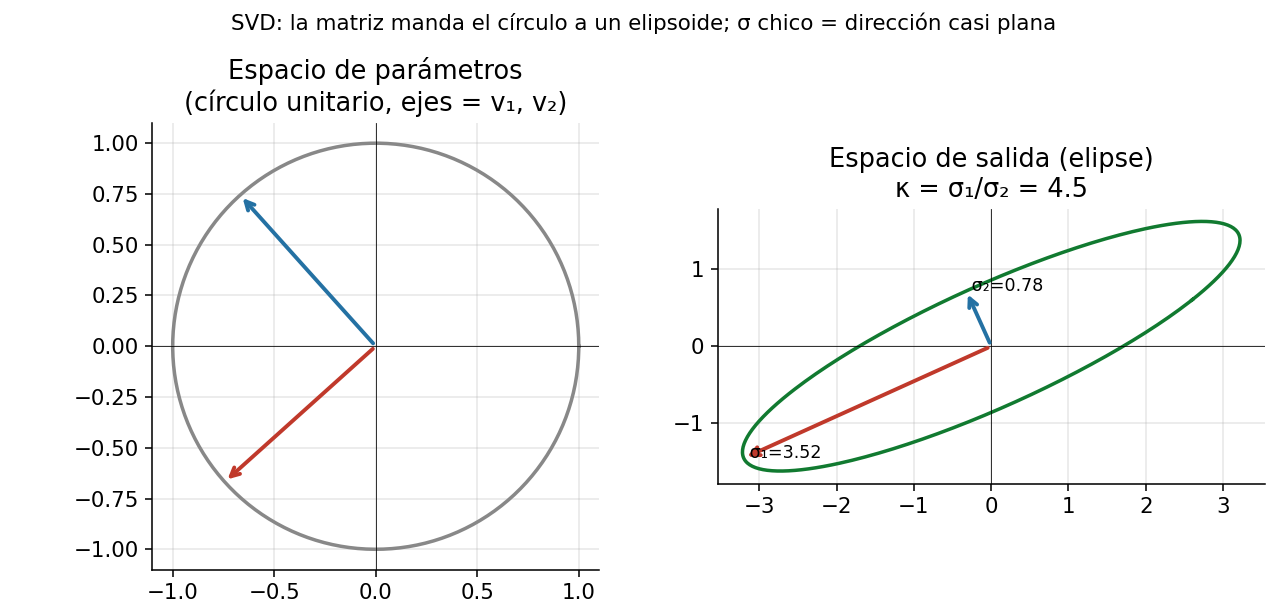
\includegraphics[width=0.75\linewidth]{fig_elipse_svd.png}
\caption{Una matriz transforma el círculo unitario en una elipse: los ejes de la elipse son las direcciones propias (vectores singulares) y sus longitudes son los valores singulares. Una elipse muy alargada corresponde a una forma cuadrática mal condicionada, con una dirección ``dura'' y una ``blanda''. Esta es la geometría del ``valle plano'' del error. (figura del proyecto)}
\label{fig:elipse}
\end{figure}

\textbf{Por qué en este proyecto.} Cerca del óptimo, el error se comporta como una forma cuadrática cuya matriz es el Hessiano ($\approx$ FIM). Entonces las curvas de nivel del error son elipsoides. Si un eje es larguísimo (autovalor casi nulo), tenemos el \textbf{valle plano}: podés recorrer esa dirección sin que el error cambie. Esa dirección larga es, en nuestro modelo, la que involucra a $w_{II}$: mover $w_{II}$ casi no encarece el ajuste, y por eso los datos no lo fijan bien.

\emph{En el proyecto esto reaparece en:} M6, donde ``valle plano'' $=$ elipsoide de error con un eje muy largo $=$ autovalor chico de la FIM.

\section{Normas, ortogonalidad y número de condición}

\begin{definition}[Normas]
La \textbf{norma euclídea} de un vector es $\|\mathbf{v}\|_2=\sqrt{\mathbf{v}\transp\mathbf{v}}$. Para matrices, la \textbf{norma espectral} $\|A\|_2$ es el mayor valor singular de $A$ (cuánto puede estirar como máximo a un vector unitario).
\end{definition}

\textbf{Ortogonalidad.} Dos vectores son ortogonales si $\mathbf{u}\transp\mathbf{v}=0$. Una matriz $Q$ es \textbf{ortogonal} si $Q\transp Q=I$: representa una rotación/reflexión pura (no cambia longitudes ni ángulos). Los autovectores de una matriz simétrica se pueden elegir ortonormales, y esa base ortogonal es la que ``endereza'' la geometría del problema.

\begin{definition}[Número de condición]
Para una matriz $A$ con valores singulares $\sigma_{\max}\ge\dots\ge\sigma_{\min}$, el \textbf{número de condición} es
\[
\kappa(A)=\frac{\sigma_{\max}}{\sigma_{\min}}.
\]
Si $A$ es simétrica definida positiva, equivale a $\lambda_{\max}/\lambda_{\min}$.
\end{definition}

\textbf{Intuición.} $\kappa$ mide qué tan ``estirado'' es el elipsoide: $\kappa=1$ es una esfera perfecta (bien condicionado); $\kappa$ enorme es una elipse casi degenerada (mal condicionado). Un problema mal condicionado es sensible al ruido y difícil de optimizar: el descenso por gradiente rebota de pared a pared del valle en vez de avanzar hacia el fondo, como muestra la Figura~\ref{fig:valle}.

\begin{figure}[H]
\centering
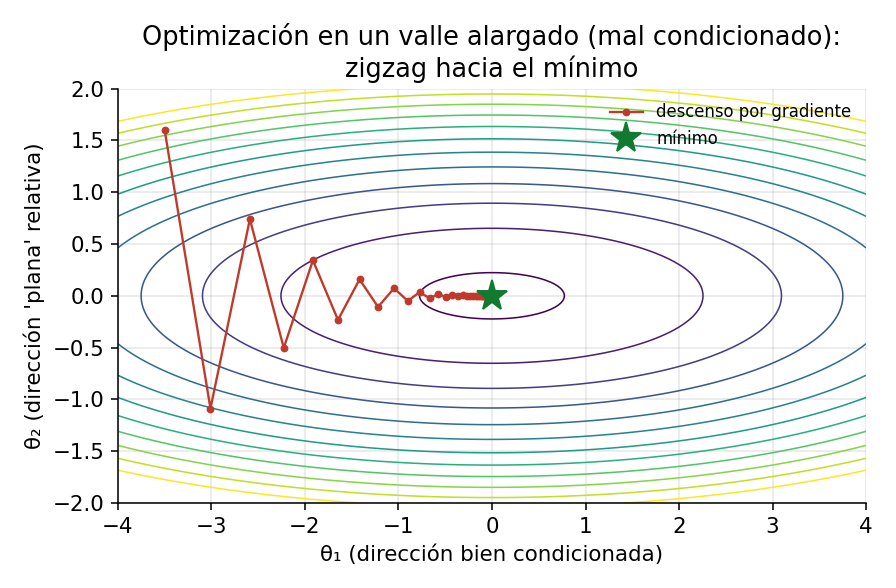
\includegraphics[width=0.75\linewidth]{fig_gradiente_valle.png}
\caption{Descenso por gradiente en un valle mal condicionado (número de condición $\kappa$ grande): las curvas de nivel forman una elipse alargada y el gradiente zigzaguea entre las paredes en lugar de ir directo al mínimo. Cuanto mayor es $\kappa$, más lento y ruidoso el ajuste. (figura del proyecto)}
\label{fig:valle}
\end{figure}

\textbf{Por qué en este proyecto.} El número de condición de la FIM es \emph{la} métrica de identificabilidad del proyecto: un $\kappa$ enorme dice que hay una dirección de parámetros casi invisible para los datos. El diseño óptimo de experimentos (OED) busca justamente estímulos $P(t),Q(t)$ que \emph{bajen} $\kappa$ de la FIM, redondeando el elipsoide para que $w_{II}$ deje de ser un valle plano.

\emph{En el proyecto esto reaparece en:} M6 y en el OED (elegir el estímulo que minimiza $\kappa$ de la FIM); también explica por qué el entrenamiento sufre cuando el problema está mal condicionado.

\section{Serie de Taylor de segundo orden}

\begin{definition}[Aproximación cuadrática]
Alrededor de un punto $\thetavec_0$, una función escalar suave se aproxima como
\[
f(\thetavec)\approx f(\thetavec_0)+\nabla f(\thetavec_0)\transp(\thetavec-\thetavec_0)+\tfrac12(\thetavec-\thetavec_0)\transp H(\thetavec_0)\,(\thetavec-\thetavec_0),
\]
con $H$ el Hessiano evaluado en $\thetavec_0$.
\end{definition}

\textbf{Intuición.} Es la generalización a varias variables de la parábola que aproxima una curva. El término lineal usa el gradiente; el término cuadrático usa el Hessiano y fija la \emph{forma} de la superficie.

\textbf{Por qué en este proyecto.} Este es el broche que une todo lo anterior. En el óptimo del ajuste, $\thetavec^\star$, el gradiente se anula ($\nabla L(\thetavec^\star)=\bm0$), así que el término lineal desaparece y queda
\[
L(\thetavec)\approx L(\thetavec^\star)+\tfrac12(\thetavec-\thetavec^\star)\transp H\,(\thetavec-\thetavec^\star).
\]
El error, cerca del óptimo, es \emph{exactamente} una forma cuadrática cuya matriz es el Hessiano ($\approx$ FIM). Entonces:
\begin{itemize}[nosep]
  \item las curvas de nivel del error son elipsoides (Sección 5);
  \item los ejes son los autovectores de $H$ y sus longitudes van como $1/\sqrt{\lambda_i}$ (Sección 4);
  \item un autovalor chico $=$ eje largo $=$ valle plano $=$ parámetro mal identificado ($w_{II}$).
\end{itemize}
Todo el diagnóstico de identificabilidad del proyecto vive en este único desarrollo de Taylor de segundo orden.

\emph{En el proyecto esto reaparece en:} M6, como la justificación formal de por qué la FIM/Hessiano describe la incertidumbre de los parámetros y por qué $w_{II}$ cae en el valle plano.

\section*{Síntesis}
\addcontentsline{toc}{section}{Síntesis}

El hilo conductor es corto: el \textbf{gradiente} entrena, el \textbf{Jacobiano} $J=\partial\mathbf{y}/\partial\thetavec$ es la sensibilidad (M5), y el \textbf{Hessiano}/FIM $\approx J\transp J$ describe la curvatura del error (M6). Diagonalizándolo obtenemos autovalores (información por dirección) y su cociente extremo, el \textbf{número de condición} $\kappa$. Un $\kappa$ grande significa un elipsoide de error muy alargado --- el ``valle plano'' --- y ahí es donde $w_{II}$ se vuelve inidentificable. El desarrollo de Taylor de segundo orden es lo que conecta ``error'' con ``forma cuadrática'' y cierra el argumento.

\begin{thebibliography}{9}
\bibitem{strang} G. Strang, \emph{Linear Algebra and Its Applications}, Harcourt Brace Jovanovich, 3.ª ed., 1988.
\bibitem{golub} G. H. Golub y C. F. Van Loan, \emph{Matrix Computations}, Johns Hopkins University Press, 4.ª ed., 2013.
\end{thebibliography}

\end{document}
